\documentclass{beamer}
\usepackage{tcolorbox}
\usepackage{hyperref}
\usepackage{booktabs}
\usepackage{siunitx}
\usepackage{tikz}
\usepackage{forest}
\usetikzlibrary{positioning}
\newdimen\nodeDist
\nodeDist=33mm
\usepackage{pgfplots}
\pgfplotsset{width=6cm,compat=1.9}
\usepackage{subfig}







%\beamerdefaultoverlayspecification{<+->}
% \newcommand{\data}{\mathcal{D}}
% \newcommand\Item[1][]{%
% 	\ifx\relax#1\relax  \item \else \item[#1] \fi
% 	\abovedisplayskip=0pt\abovedisplayshortskip=0pt~\vspace*{-\baselineskip}}

\graphicspath{ {imgs/} }

\usetheme{metropolis}           % Use metropolis theme


\title{Decision Trees II and Bias/Variance and Cross-Validation}
\date{\today}
\author{Nipun Batra and teaching staff}
\institute{IIT Gandhinagar}

\begin{document}
	\maketitle
	
	




\section{Real Input Real Output}

\begin{frame}{Example 1}
Let us consider the dataset given below
\begin{center}
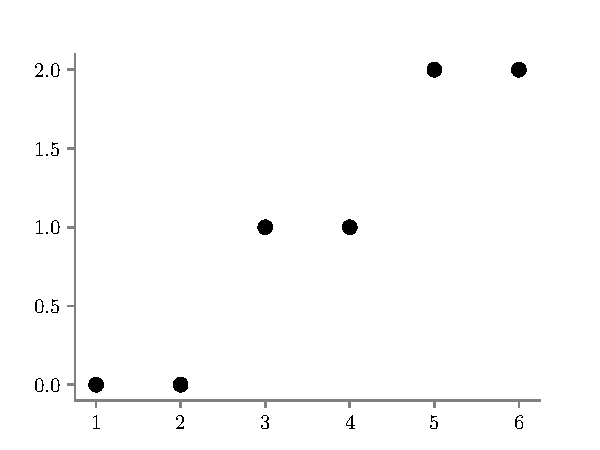
\includegraphics{../figures/decision-trees/ri-ro-dataset.pdf}
\end{center}
\end{frame}

\begin{frame}{Example 1}
What would be the prediction for decision tree with depth 0?
\begin{center}
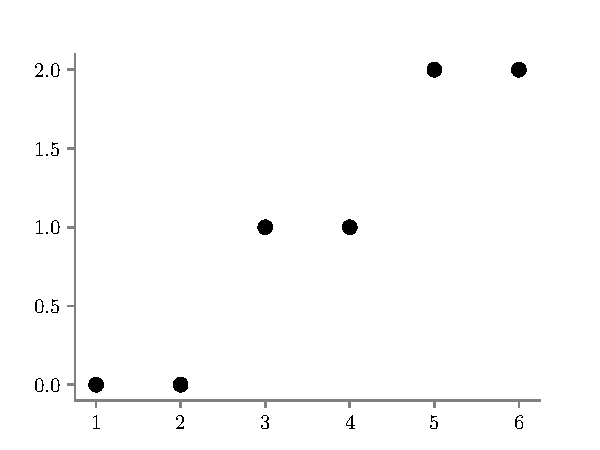
\includegraphics{../figures/decision-trees/ri-ro-dataset.pdf}
\end{center}
\end{frame}

\begin{frame}{Example 1}
Prediction for decision tree with depth 0.\\
Horizontal dashed line shows the predicted $Y$ value. It is the average of $Y$ values of all datapoints.\\
\begin{center}
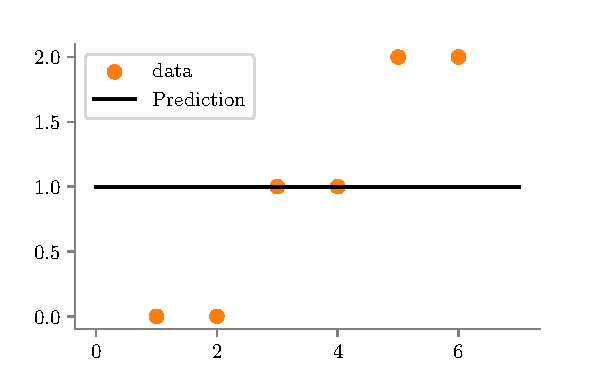
\includegraphics{../figures/decision-trees/ri-ro-depth-0.pdf}	
\end{center}
\end{frame}


\begin{frame}{Example 1}
What would be the decision tree with depth 1?
\begin{center}
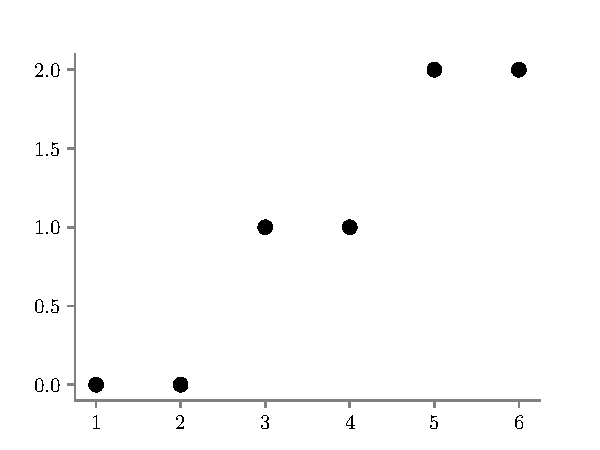
\includegraphics{../figures/decision-trees/ri-ro-dataset.pdf}
\end{center}
\end{frame}

\begin{frame}{Example 1}
Decision tree with depth 1
\begin{center}
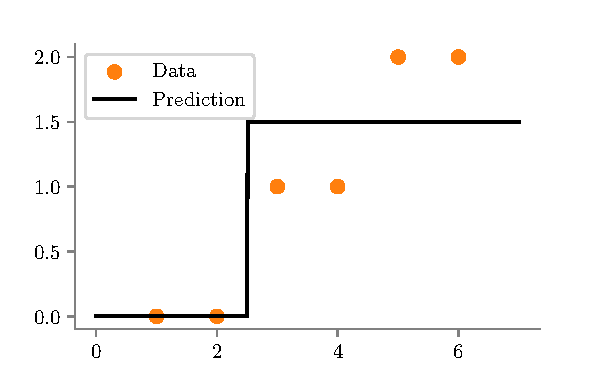
\includegraphics{../figures/decision-trees/ri-ro-depth-1.pdf}	
\end{center}
\end{frame}

\begin{frame}{Example 1}
The Decision Boundary
\begin{center}
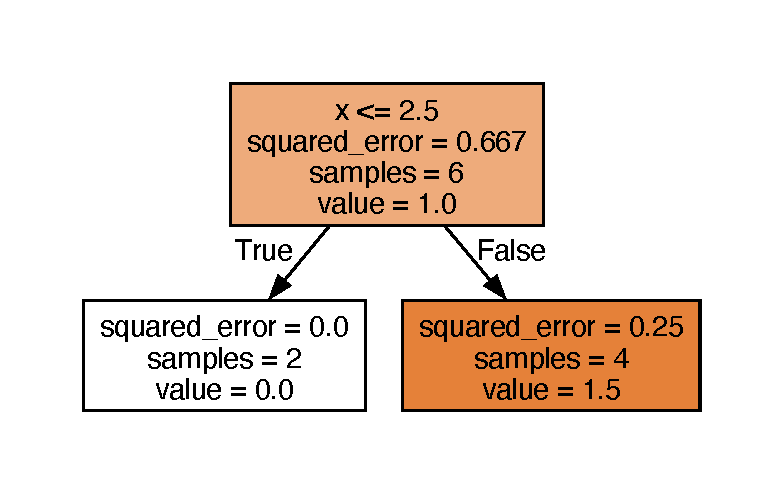
\includegraphics{../figures/decision-trees/ri-ro-depth-1-sklearn.pdf}
\end{center}
\end{frame}


\begin{frame}{Example 1}
What would be the decision tree with depth 2	?
\begin{center}
	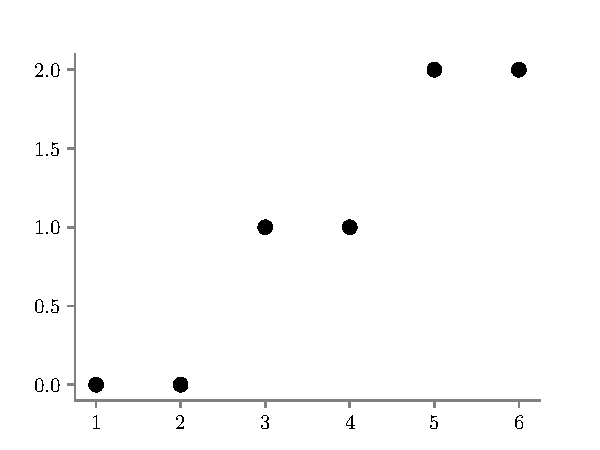
\includegraphics{../figures/decision-trees/ri-ro-dataset.pdf}
\end{center}
\end{frame}

\begin{frame}{Example 1}
	Decision tree with depth 1
	\begin{center}
	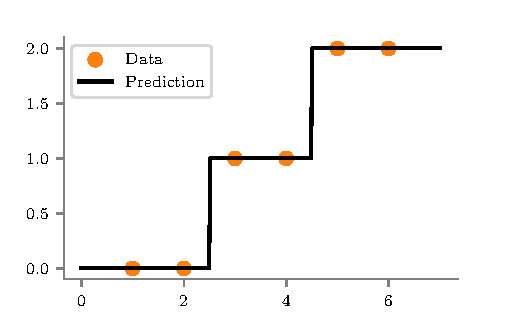
\includegraphics{../figures/decision-trees/ri-ro-depth-2.pdf}	
	\end{center}
	\end{frame}
	
	\begin{frame}{Example 1}
	The Decision Boundary
	\begin{center}
	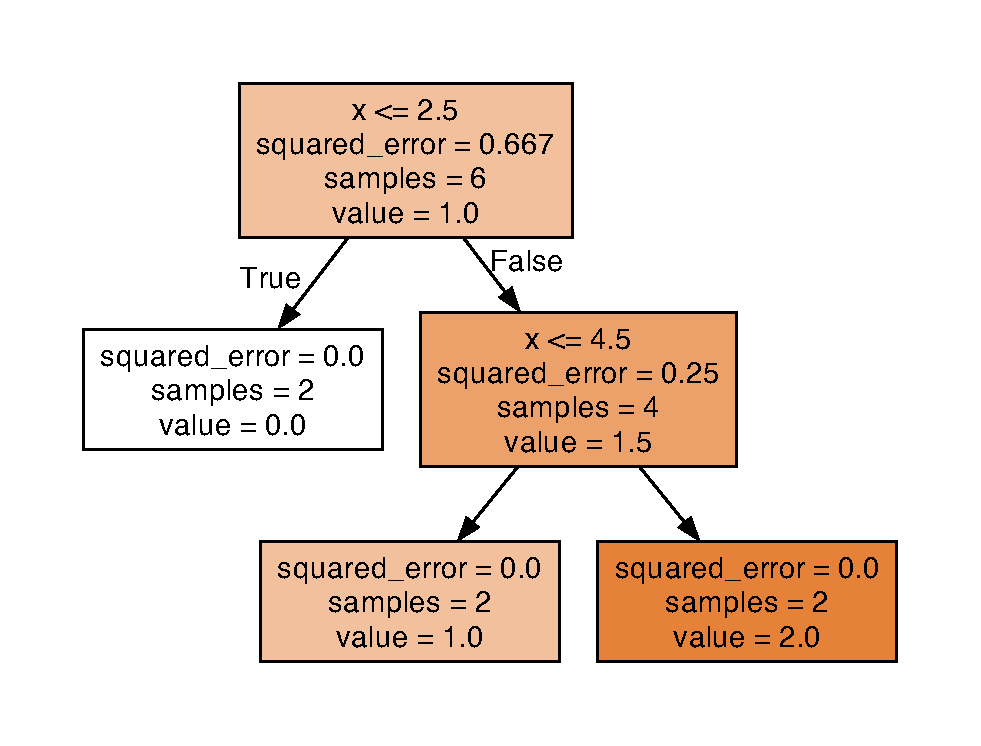
\includegraphics{../figures/decision-trees/ri-ro-depth-2-sklearn.pdf}
	\end{center}
	\end{frame}
	

\begin{frame}{Objective function}
\only<1-4>{
Here,  Feature is denoted by X and Label by Y.\\
Let the ``decision boundary'' or ``split" be at X = S.\\
Let the region X $<$ S, be region R$_1$.\\
Let the region X $>$ S, be region R$_2$.\\
\vspace{1cm}
}
\only<2-4>{
Then, let \\
$C_1$ = Mean ($Y_i | X_i \in R_1$) \\
$C_2$ = Mean ($Y_i | X_i \in R_2$) \\
}
\only<3-4>{
Loss = $\sum\limits_i$(($Y_i - C_1 | X_i \in R_1$)$^2 $ +  ($Y_i - C_2 | X_i \in R_2$)$^2 $)\\
\vspace{1cm}
}
\only<4>{
Our objective is to minimize the loss and find\\
$min_S $ $\sum\limits_i\left((Y_i - C_1 | X_i \in R_1)^2  +  (Y_i - C_2 | X_i \in R_2)^2 \right)$
}
\end{frame}

\begin{frame}{How to find optimal split ``S"?}
\end{frame}


\begin{frame}{How to find optimal split ``S"?}
\begin{enumerate}
\only<1-2>{
\item Sort all datapoints (X,Y) in increasing order of X.
\vspace{0.5cm}
}
\only<2>{
\item Evaluate the loss function for all\\
\vspace{0.25cm}
\begin{center}
$S = \frac{X_i + X_{i+1}}{2}$\\
\end{center}
\vspace{0.25cm}
and the select the S with minimum loss.
}
\end{enumerate} 
\end{frame}

\begin{frame}{A Question!}
Draw a regression tree for Y = sin(X), $0 \leq X \leq 2\pi$ 
\end{frame}

\begin{frame}{A Question!}
Dataset of Y = sin(X), $0 \leq X \leq 7$ with 10,000 points 
\begin{center}
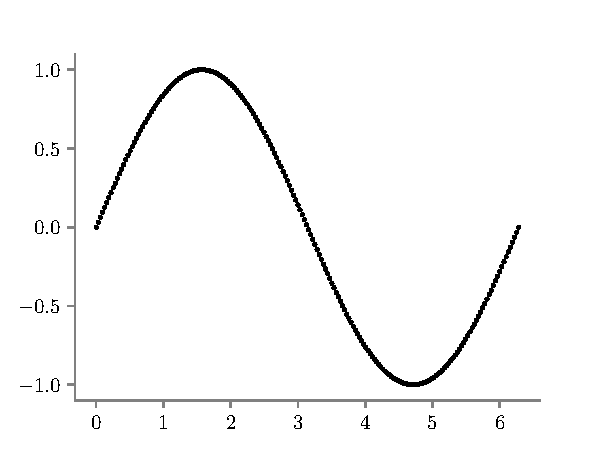
\includegraphics{../figures/decision-trees/sine-dataset.pdf}
\end{center}
\end{frame}

\begin{frame}{A Question!}
Regression tree of depth 1
\begin{center}
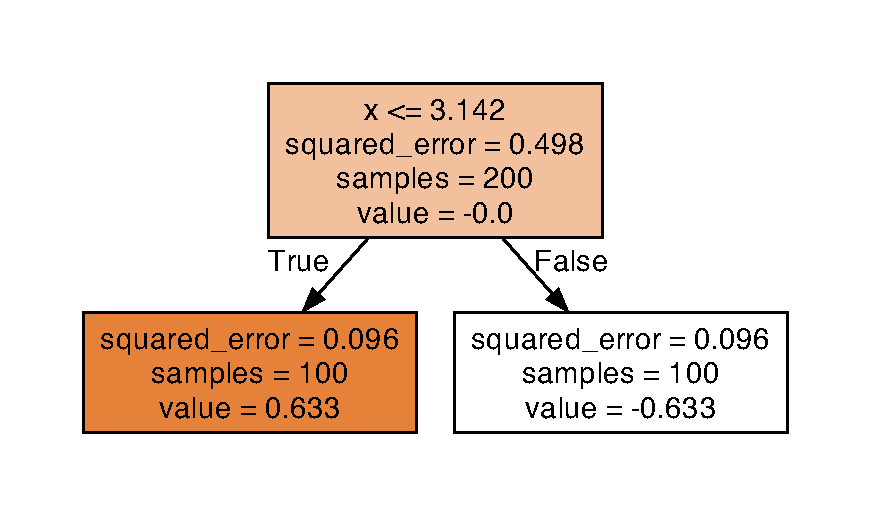
\includegraphics{../figures/decision-trees/sine-depth-1-sklearn.pdf}
\end{center}
\end{frame}

\begin{frame}{A Question!}
Decision Boundary
\begin{center}
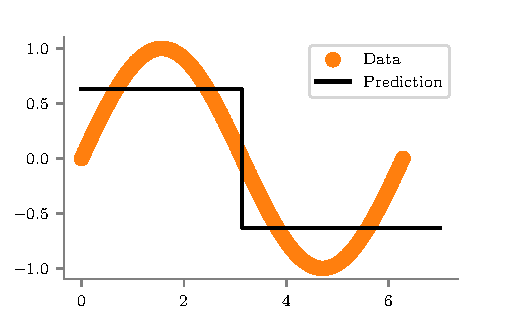
\includegraphics[scale=0.5]{../figures/decision-trees/sine-depth-1.pdf}
\end{center}
\end{frame}

\begin{frame}{A Question!}
Regression tree with no depth limit is too big to fit in a slide. \\
It has of depth 4. The decision boundaries are in figure below.\\
\begin{center}
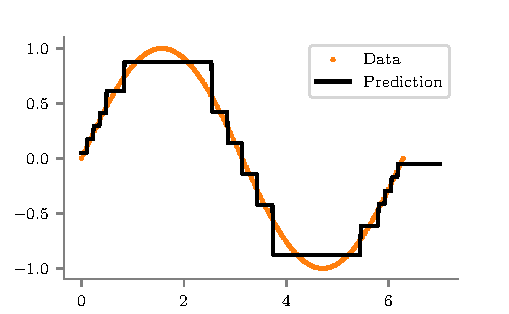
\includegraphics{../figures/decision-trees/sine-depth-4.pdf}
\end{center}
\end{frame}

\begin{frame}{Summary}
\begin{itemize}
	\item Interpretability an important goal
\item Decision trees: well known interpretable models
\item  Learning optimal tree is hard
\item  Greedy approach:
\item  Recursively split to maximize “performance gain”
\item  Issues:
\begin{itemize}
	\item Can overfit easily!
	\item  Empirically not as powerful as other methods
\end{itemize}
\end{itemize}

\end{frame}

%\begin{frame}{Code for examples}
%\begin{center}
%\href{https://colab.research.google.com/drive/1NnuVxypYfEOvpMbFHE4075CI-EkT8S7B}{Google Colab}
%\end{center}
%\end{frame}

	\begin{frame}{A Question!}
What would be the decision boundary of a decision tree classifier? 

\begin{figure}
	\centering
	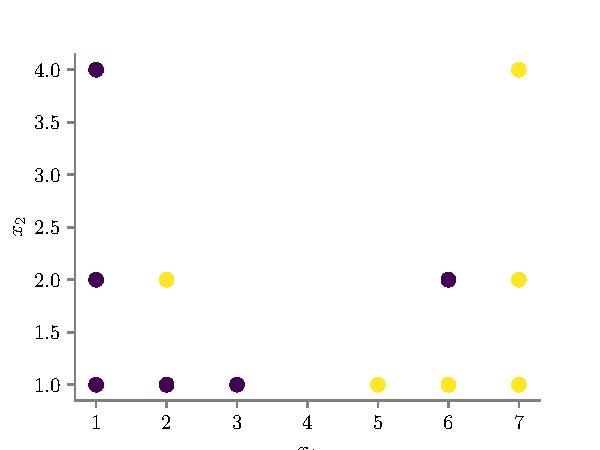
\includegraphics{../figures/decision-trees/bias-variance-dataset.pdf}
\end{figure}


\end{frame}

\begin{frame}{Decision Boundary for a tree with depth 1}
\begin{figure}%
\centering
\subfloat[Decision Boundary]{{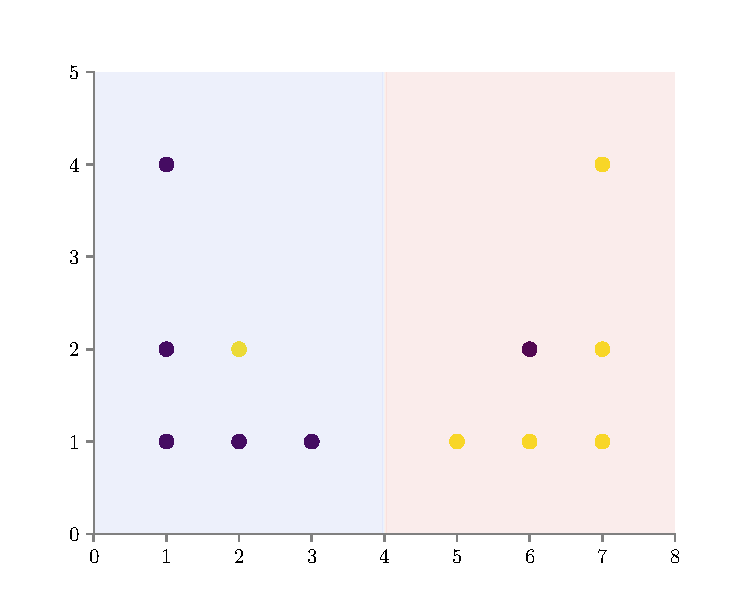
\includegraphics[width=0.45\textwidth]{../figures/decision-trees/bias-variance-depth-1.pdf} }}%
\qquad
\subfloat[Decision Tree]{{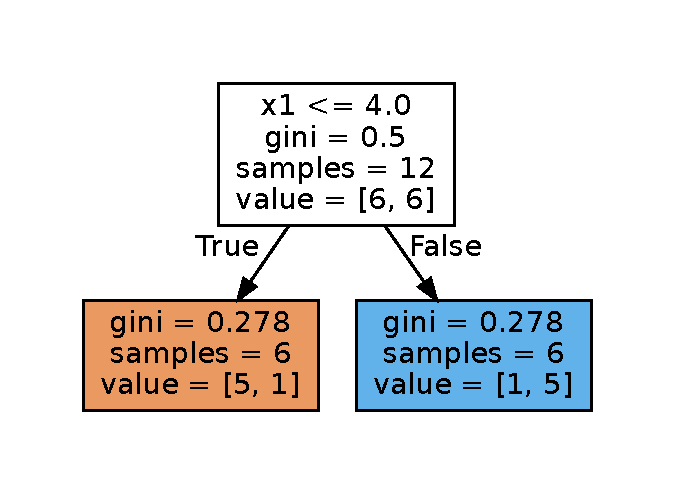
\includegraphics[width =0.45\textwidth]{../figures/decision-trees/bias-variance-depth-1-sklearn.pdf} }}%
\label{fig:example}%
\end{figure}
\end{frame}

\begin{frame}{Decision Boundary for a tree with no depth limit}
\begin{figure}%
\centering
\subfloat[Decision Boundary]{{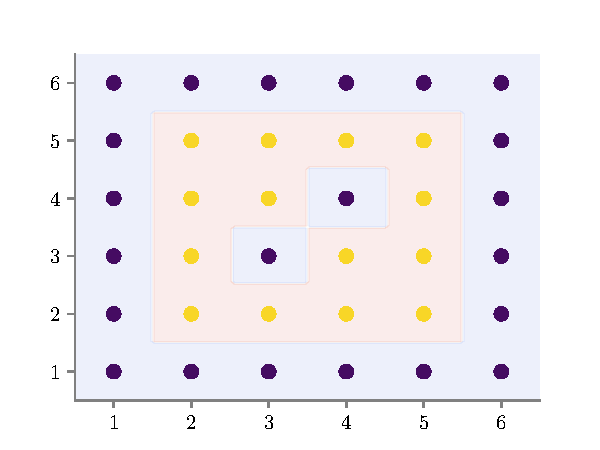
\includegraphics[width=0.45\textwidth]{../figures/decision-trees/bias-variance-full-depth.pdf} }}%
\qquad
\subfloat[Decision Tree]{{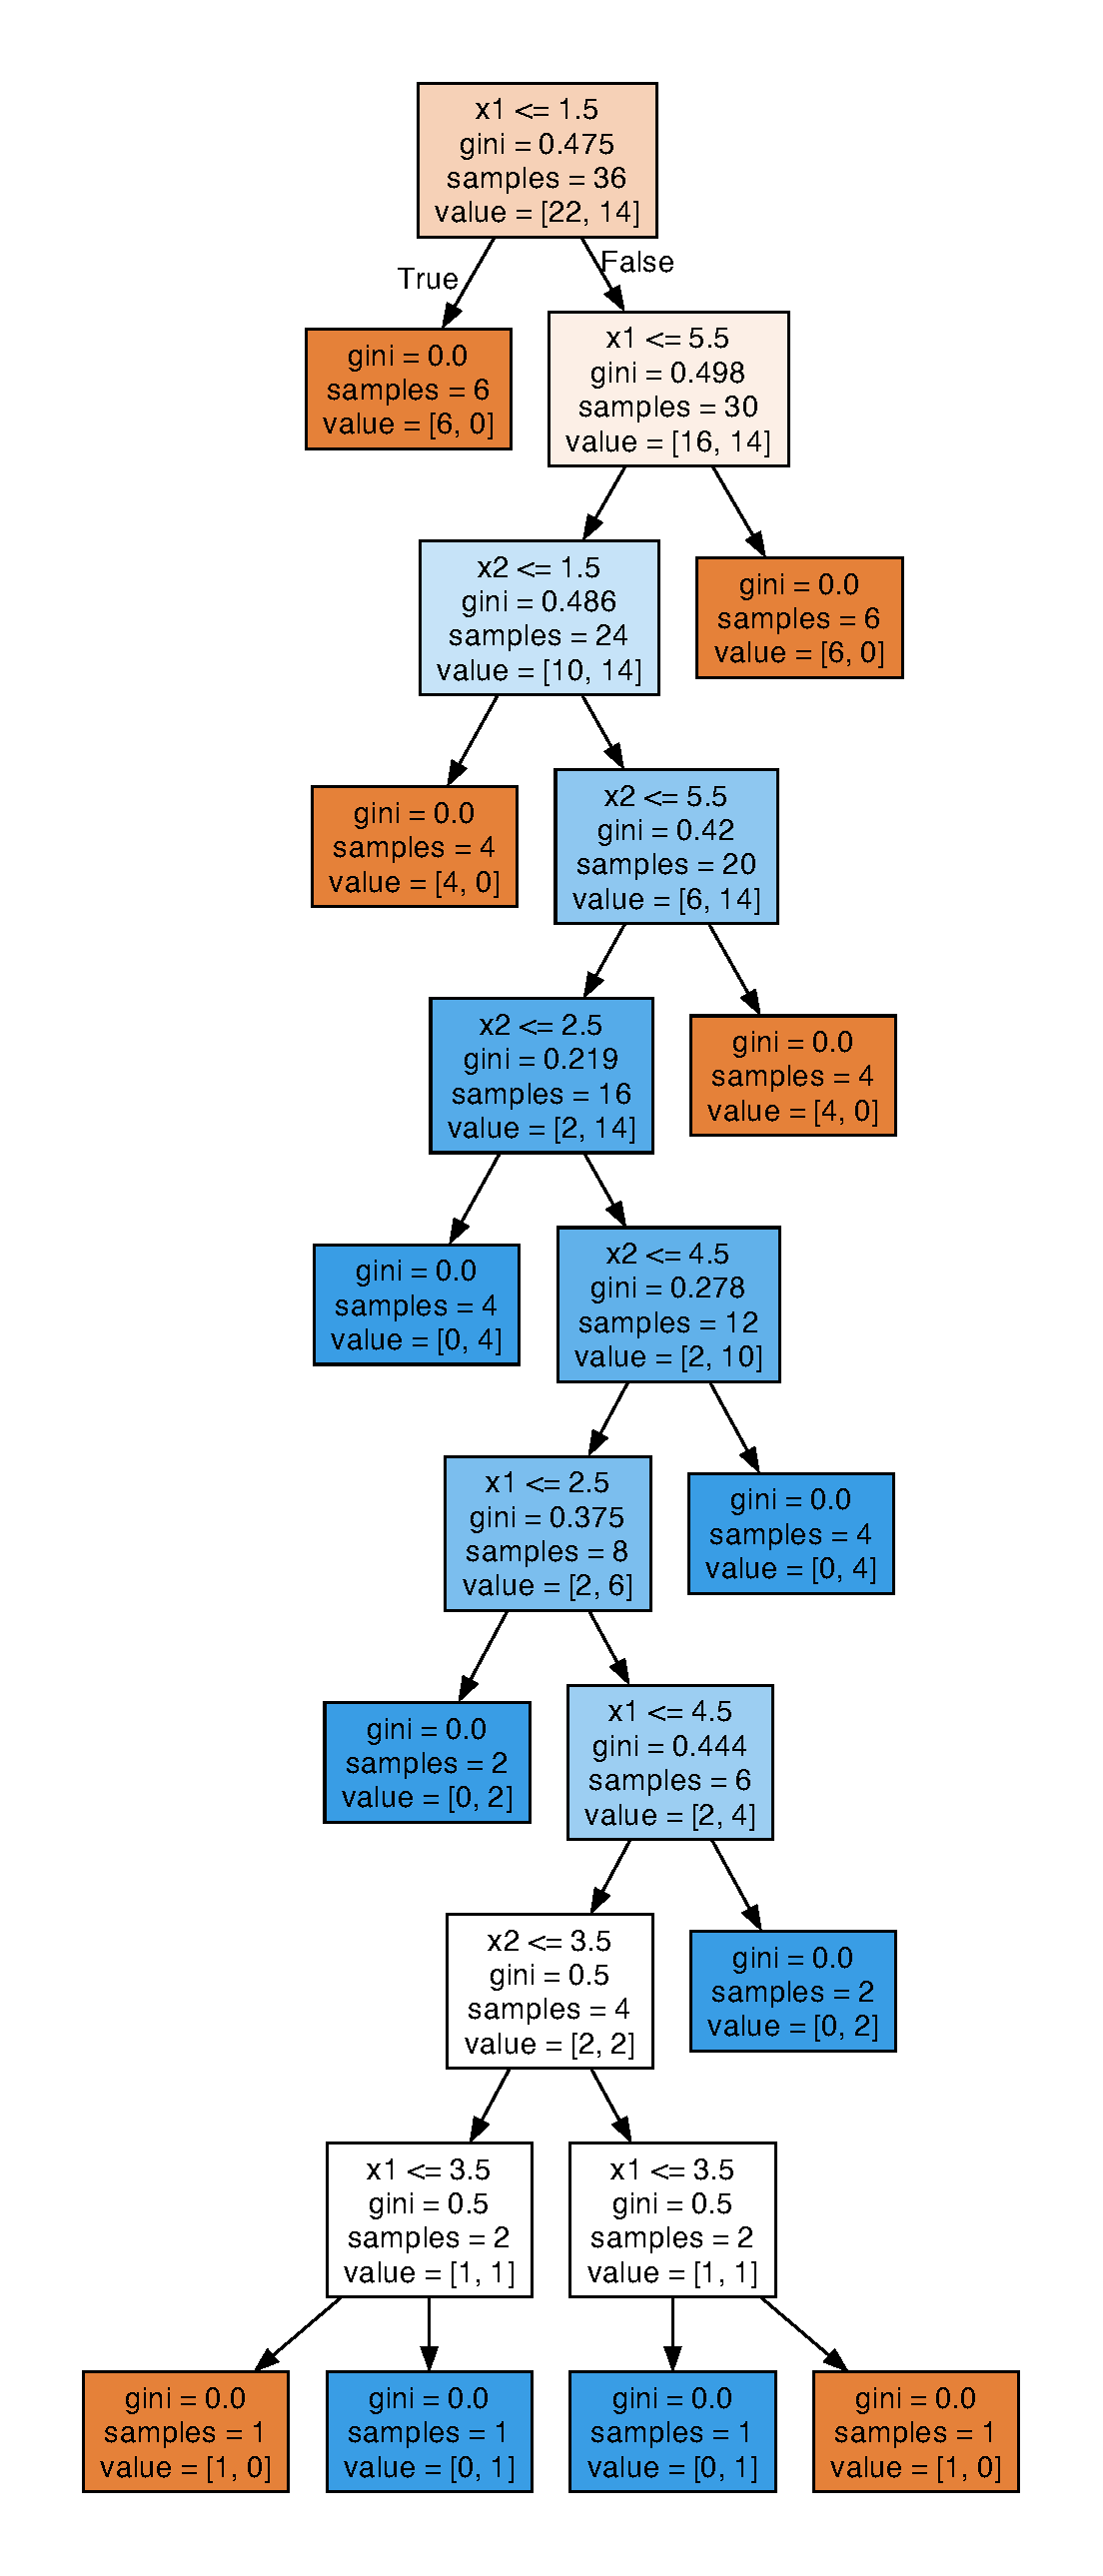
\includegraphics[width =0.45\textwidth]{../figures/decision-trees/bias-variance-full-depth-sklearn.pdf} }}%
\label{fig:example}%
\end{figure}
\end{frame}


\begin{frame}{Are deeper trees always better?}
\only<1-2>{
As we saw, deeper trees learn more complex decision boundaries.
}

\only<2>{
\vspace{1cm}
But, sometimes this can lead to $poor$ $generalization$
}	
\end{frame}

\begin{frame}{An example}
Consider the dataset below
\begin{figure}%
\centering
\subfloat[Train Set]{{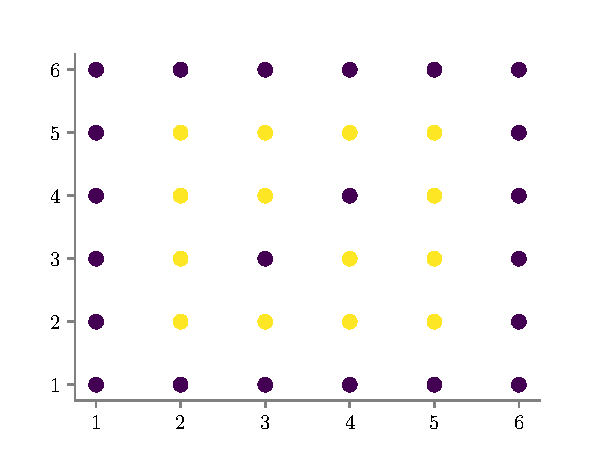
\includegraphics[width=0.45\textwidth]{../figures/decision-trees/bias-variance-dataset-2.pdf} }}%
\qquad
\subfloat[Test Set]{{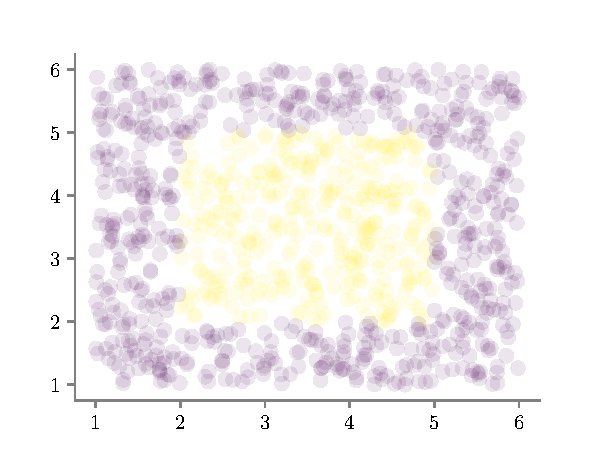
\includegraphics[width =0.45\textwidth]{../figures/decision-trees/bias-variance-dataset-2-test.pdf} }}%
\label{fig:example}%
\end{figure}
\end{frame}

\begin{frame}{Underfitting}
Underfitting is also known as $high$ $bias$, since it has a very biased incorrect assumption.
\begin{figure}%
\centering
\subfloat[Decision Boundary]{{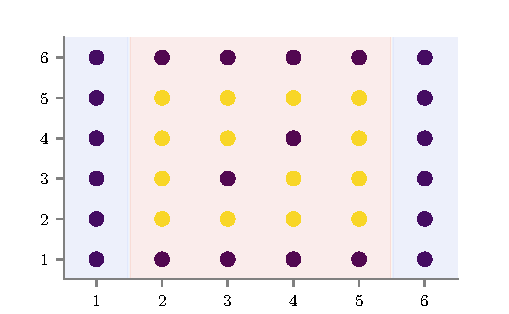
\includegraphics[width=0.45\textwidth]{../figures/decision-trees/bias-variance-depth-2.pdf} }}%
\qquad
\subfloat[Decision Tree]{{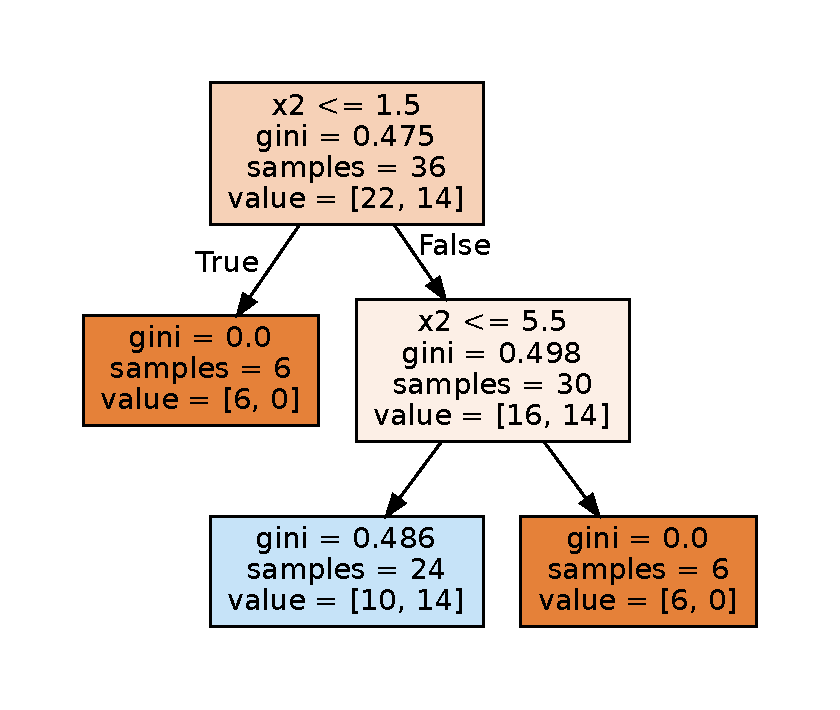
\includegraphics[width =0.45\textwidth]{../figures/decision-trees/bias-variance-depth-2-sklearn.pdf} }}%
\label{fig:example}%
\end{figure}
\end{frame}

\begin{frame}{Overfitting}
Overfitting is also known as $high$ $variance$, since very small changes in data can lead to very different models.\\
Decision tree learned has depth of 10.
\begin{center}
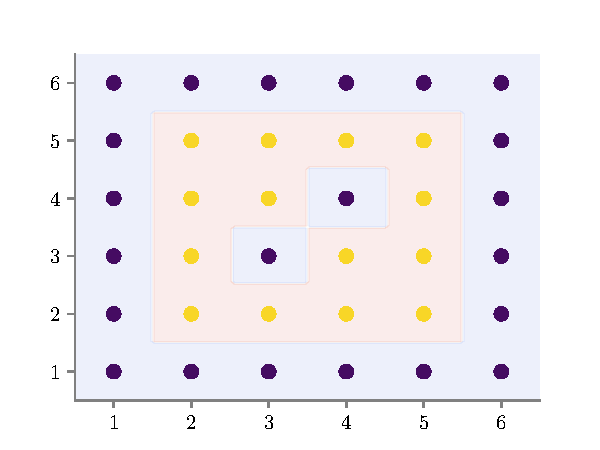
\includegraphics[scale=0.5]{../figures/decision-trees/bias-variance-full-depth.pdf}
\end{center}
\end{frame}


\begin{frame}{Intution for Variance}
A small change in data can lead to very different models.\\
\vspace{1cm}
\begin{columns}
\begin{column}{0.5\textwidth}{\hspace{1.75cm} Dataset 1}
\begin{center}
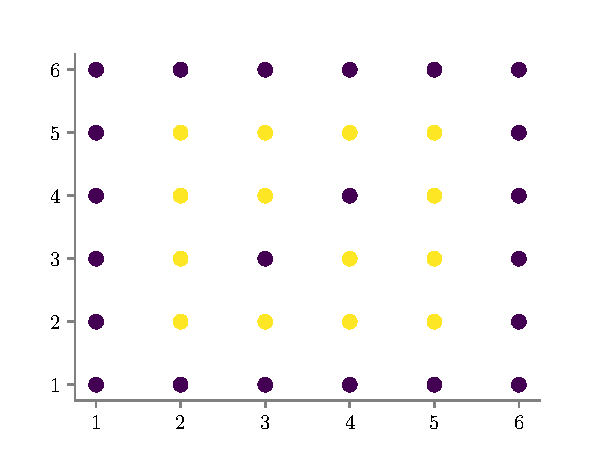
\includegraphics[width = \textwidth]{../figures/decision-trees/bias-variance-dataset-2.pdf}
\end{center}
\end{column}
\begin{column}{0.5\textwidth}{\hspace{1.75cm} Dataset 2}
\begin{center}
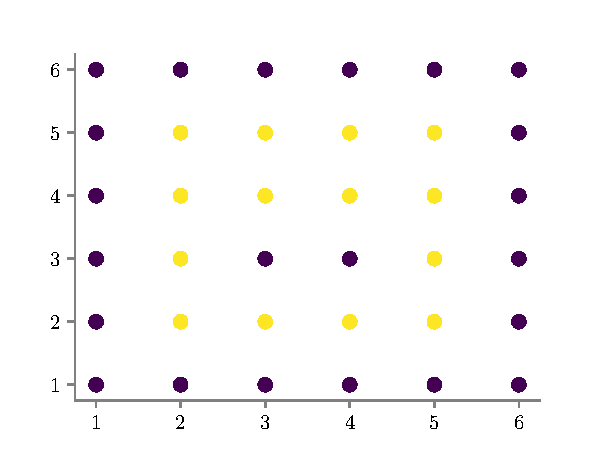
\includegraphics[width = \textwidth]{../figures/decision-trees/bias-variance-dataset-2-2.pdf}
\end{center}
\end{column}
\end{columns}
\end{frame}


\begin{frame}{Intution for Variance}
\begin{columns}
\begin{column}{0.5\textwidth}
\begin{center}
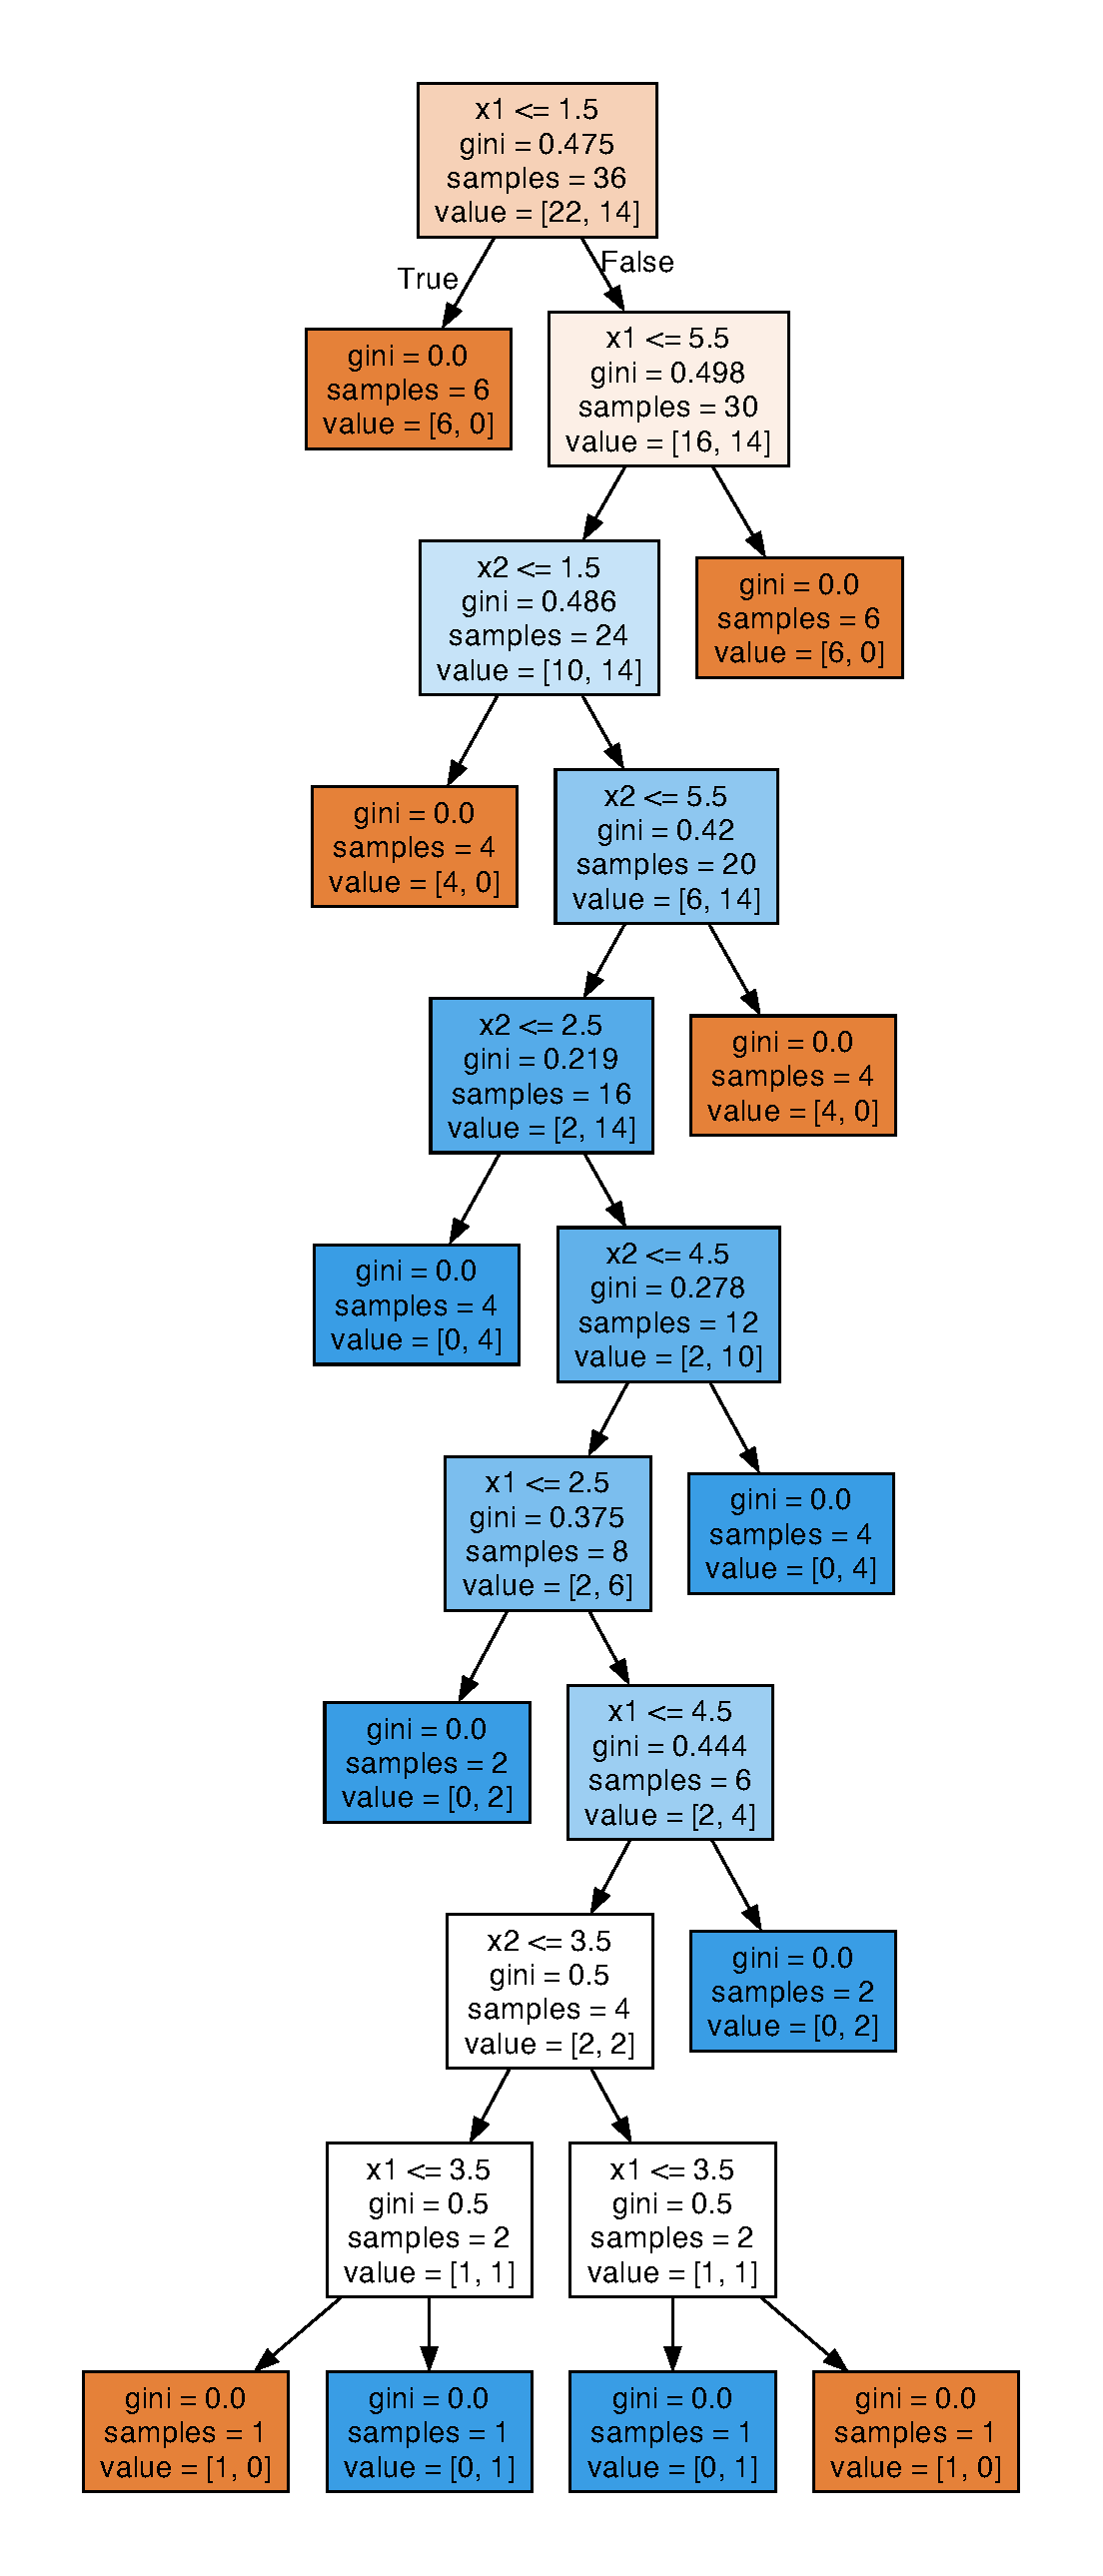
\includegraphics[scale=0.2]{../figures/decision-trees/bias-variance-full-depth-sklearn.pdf}
\end{center}
\end{column}
\begin{column}{0.5\textwidth}
\begin{center}
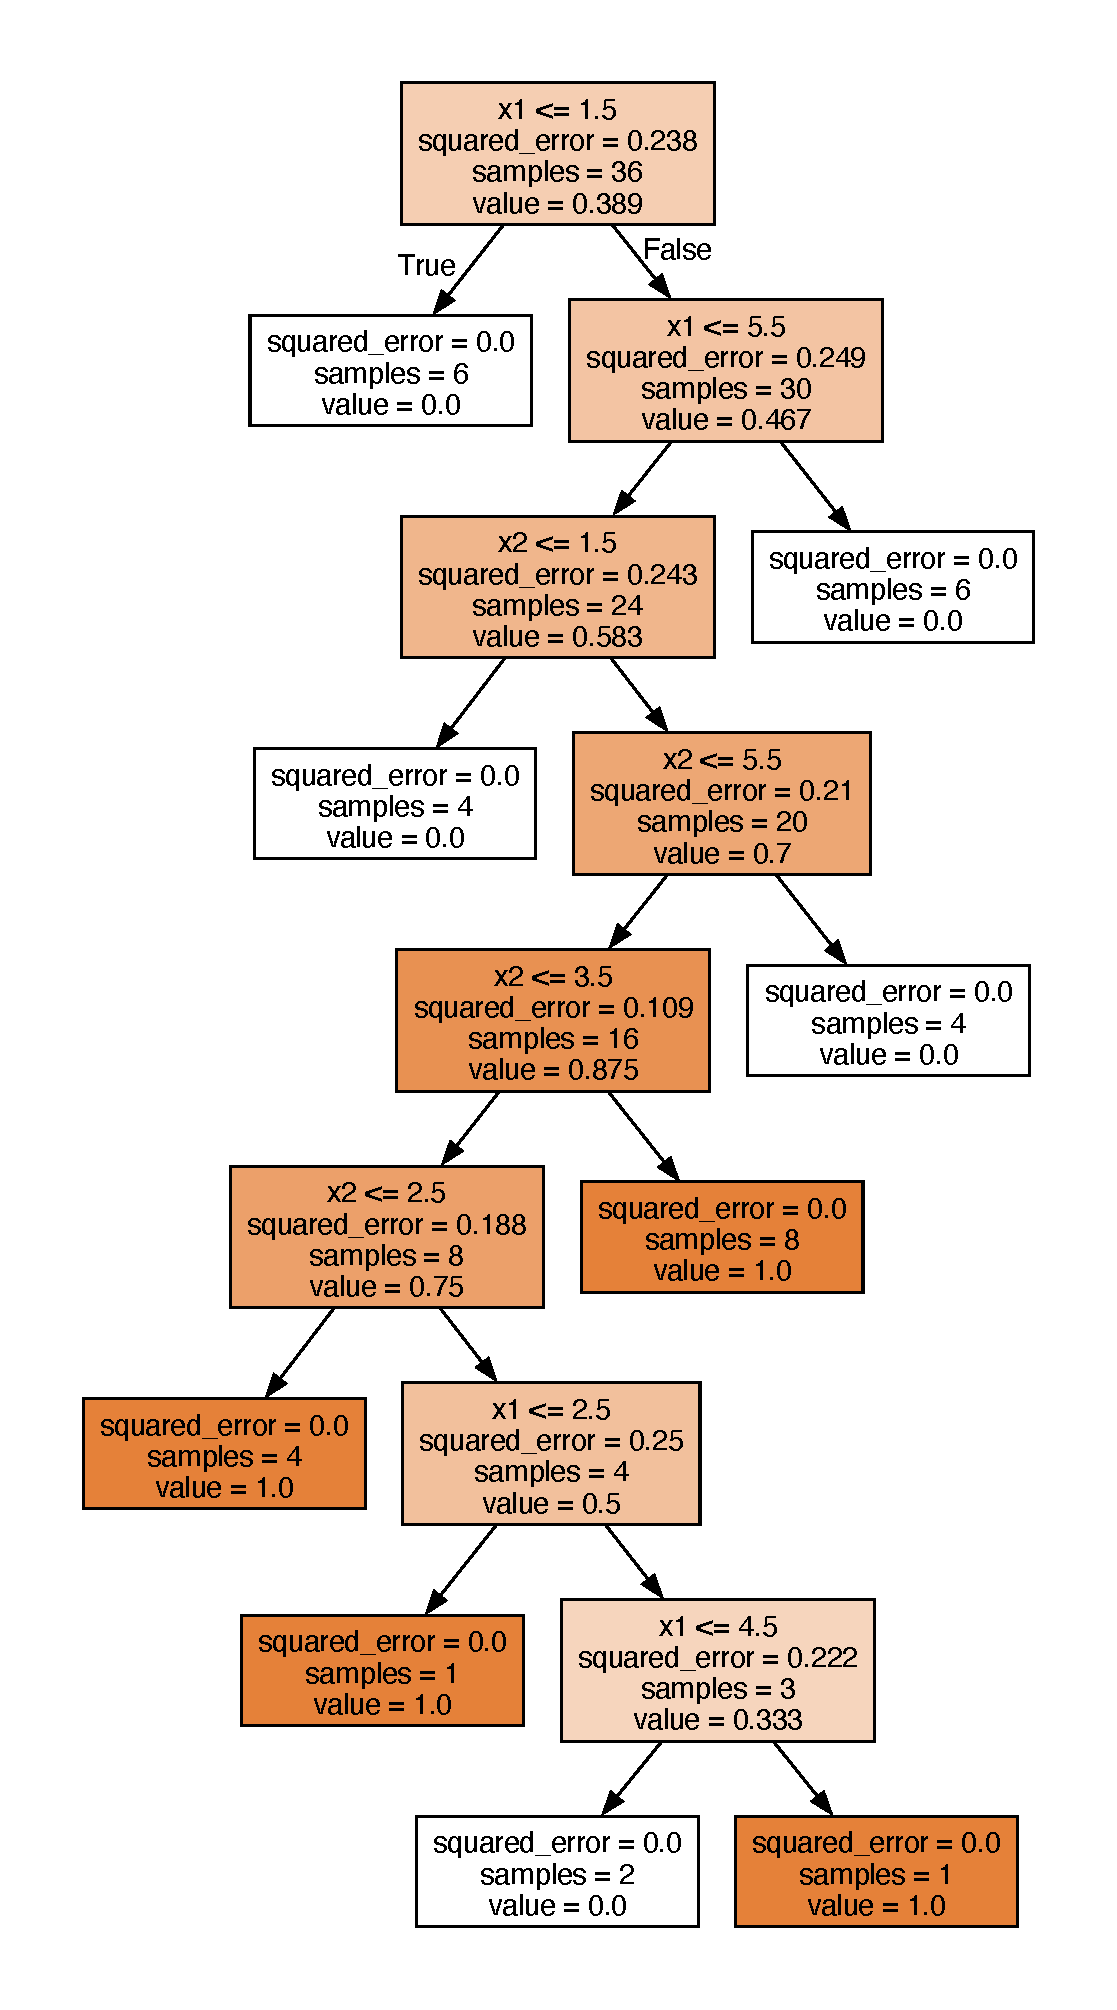
\includegraphics[scale=0.2]{../figures/decision-trees/bias-variance-full-depth-sklearn-2.pdf}
\end{center}
\end{column}
\end{columns}
\end{frame}


\begin{frame}{A Good Fit}
\begin{columns}
\begin{column}{0.5\textwidth}
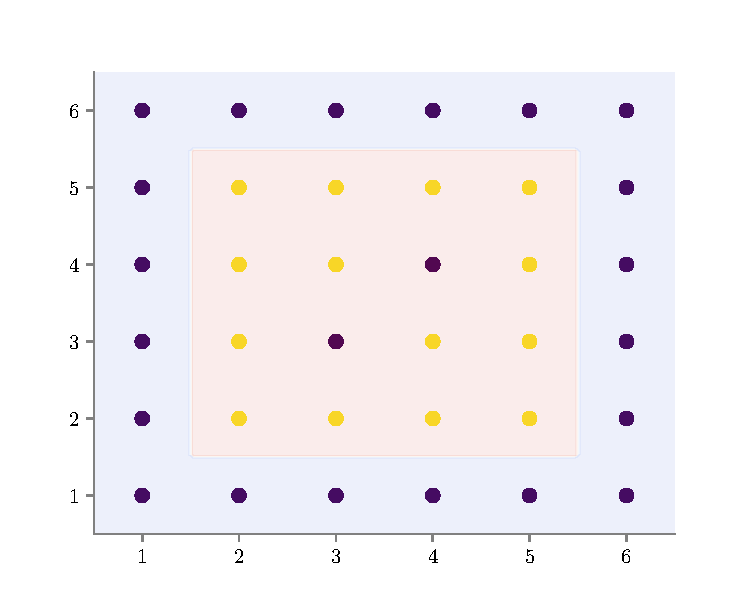
\includegraphics[width=\textwidth]{../figures/decision-trees/bias-variance-good-fit.pdf}
\end{column}
\begin{column}{0.5\textwidth}
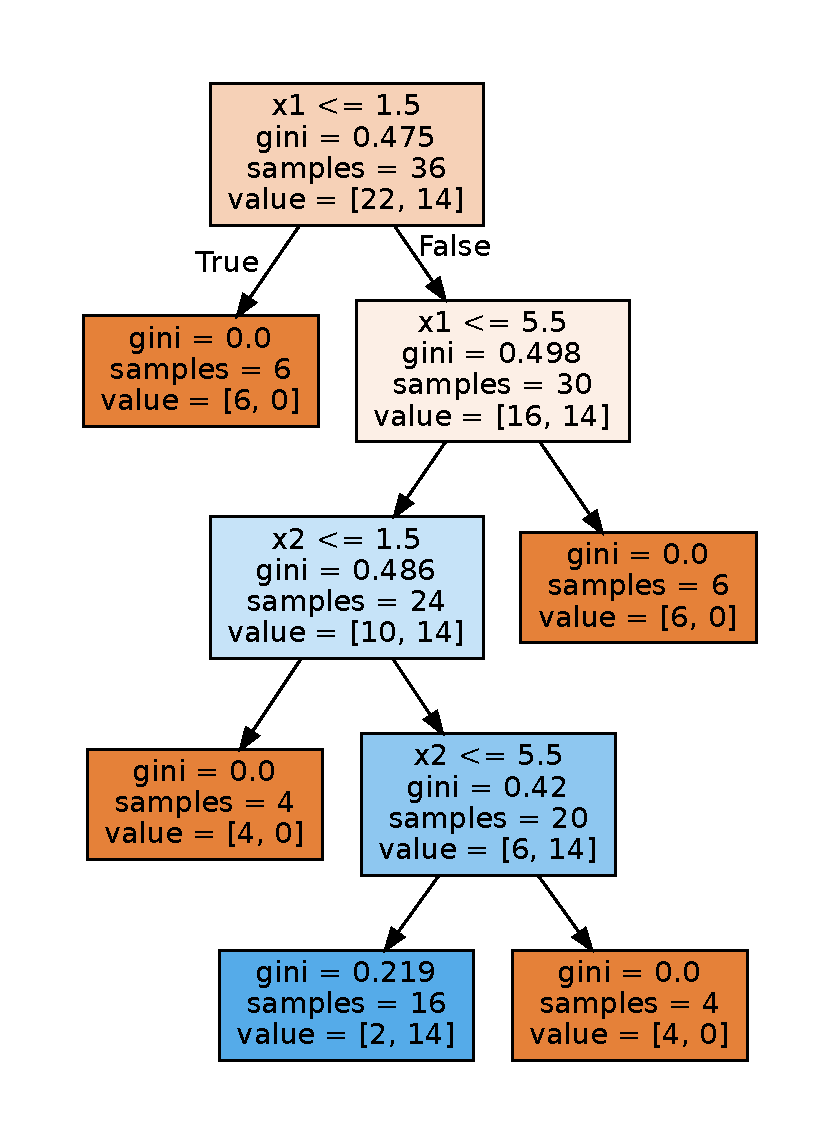
\includegraphics[width =\textwidth]{../figures/decision-trees/bias-variance-good-fit-sklearn.pdf}
\end{column}
\end{columns}

\end{frame}

\begin{frame}{Accuracy vs Depth Curve}
\begin{center}
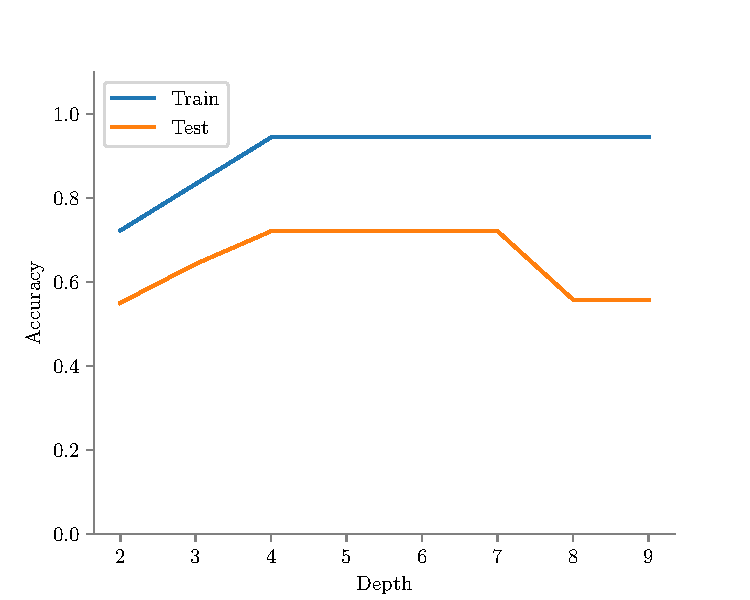
\includegraphics[scale=0.55]{../figures/decision-trees/bias-variance-accuracy-vs-depth.pdf}
\end{center}
\pause As depth increases, train accuracy improves\\
\pause As depth increases, test accuracy improves till a point\\
\pause At very high depths, test accuracy is not good (overfitting). 

\end{frame}

\begin{frame}{Accuracy vs Depth Curve : Underfitting}
The highlighted region is the underfitting region.\\
Model is too simple (less depth) to learn from the data. 
\begin{center}
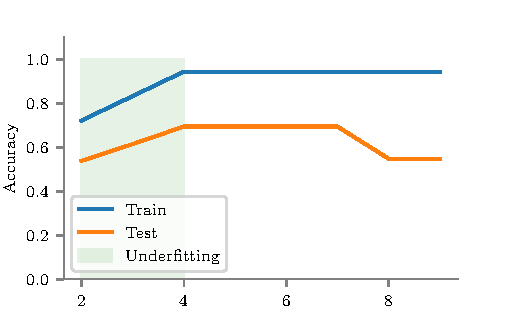
\includegraphics{../figures/decision-trees/bias-variance-accuracy-vs-depth-underfitting.pdf}
\end{center}
\end{frame}

\begin{frame}{Accuracy vs Depth Curve : Overfitting}
The highlighted region is the overfitting region.\\
Model is complex (high depth) and hence also learns the anomalies in data. 
\begin{center}
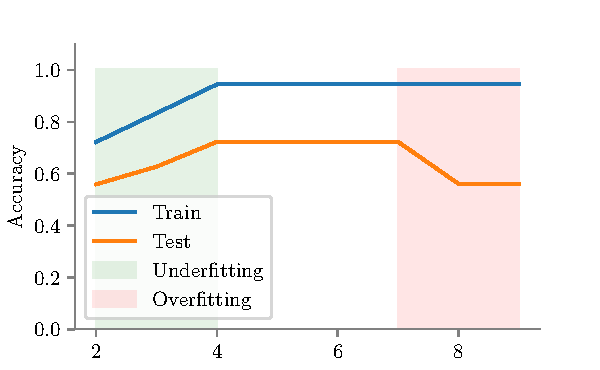
\includegraphics{../figures/decision-trees/bias-variance-accuracy-vs-depth-overfitting.pdf}
\end{center}
\end{frame}

\begin{frame}{Accuracy vs Depth Curve }
The highlighted region is the good fit region.\\
We want to maximize test accuracy while being in this region.
\begin{center}
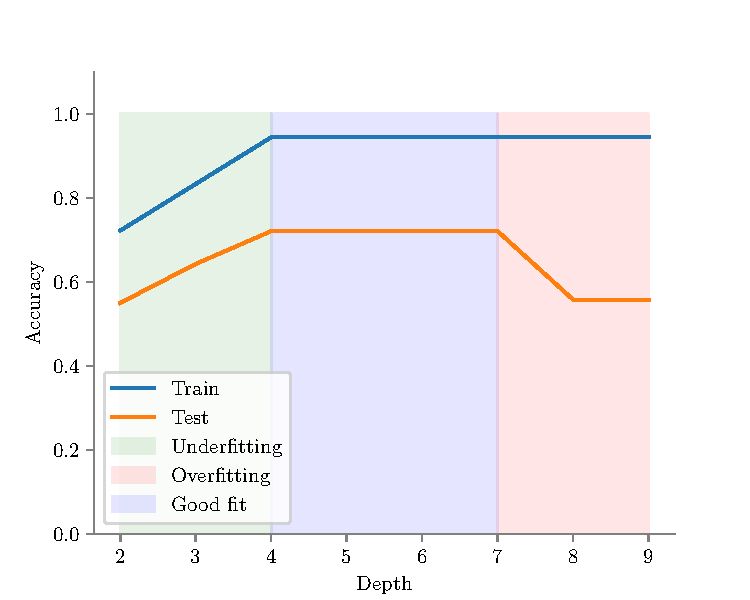
\includegraphics{../figures/decision-trees/bias-variance-accuracy-vs-depth-good-fit.pdf}
\end{center}
\end{frame}

\begin{frame}{The big question!?}
\only<1-2>{
How to find the optimal depth for a decision tree?\\
}
\only<2>{
\vspace{1cm}
Use cross-validation!
}
\end{frame}


\begin{frame}{Our General Training Flow}
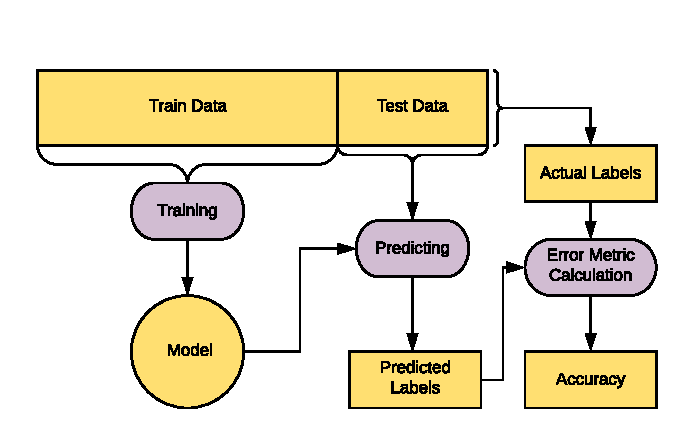
\includegraphics[width = \textwidth]{../diagrams/cross-validation/general-workflow}
\end{frame}

\begin{frame}{K-Fold cross-validation: Utilise full dataset for testing}
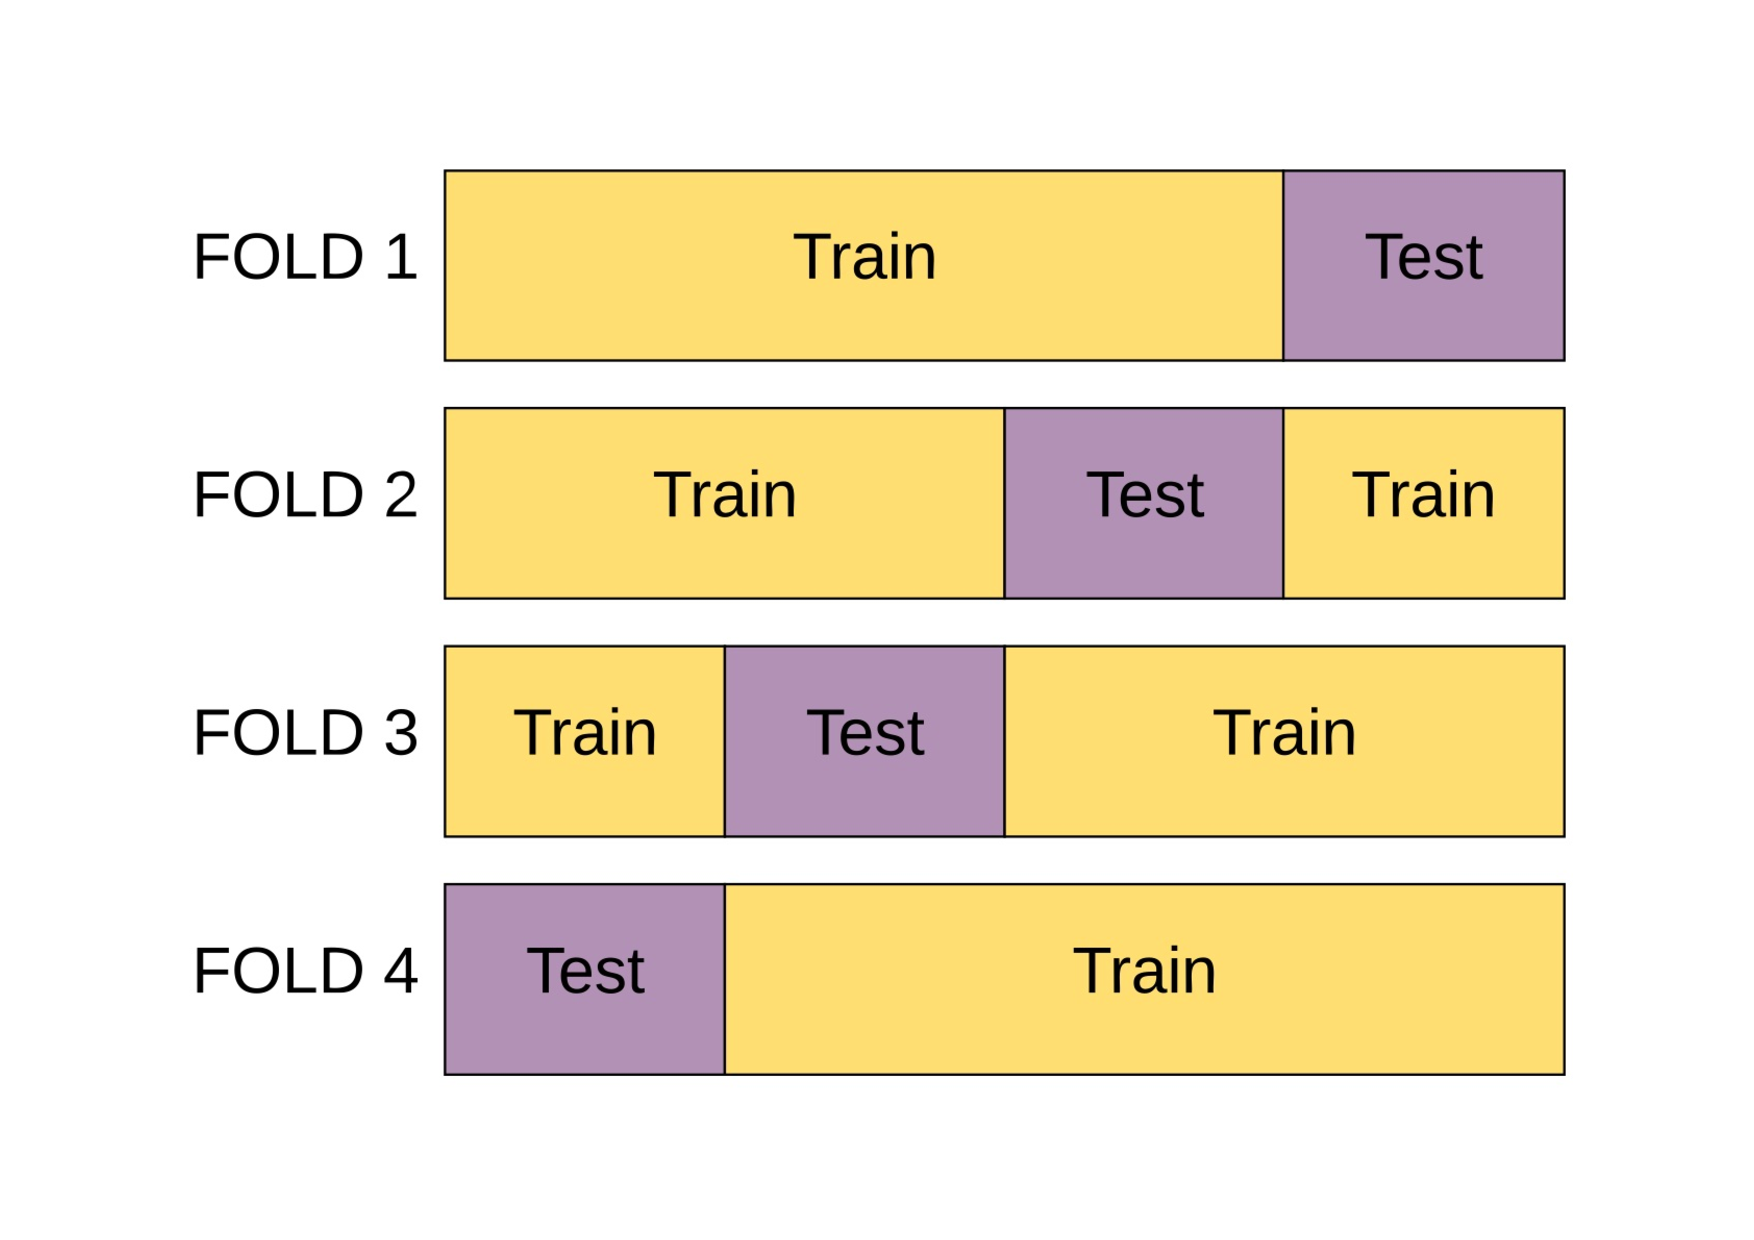
\includegraphics[width = \textwidth]{../diagrams/cross-validation/cross-validation-train-test}
\end{frame}

\begin{frame}{The Validation Set}
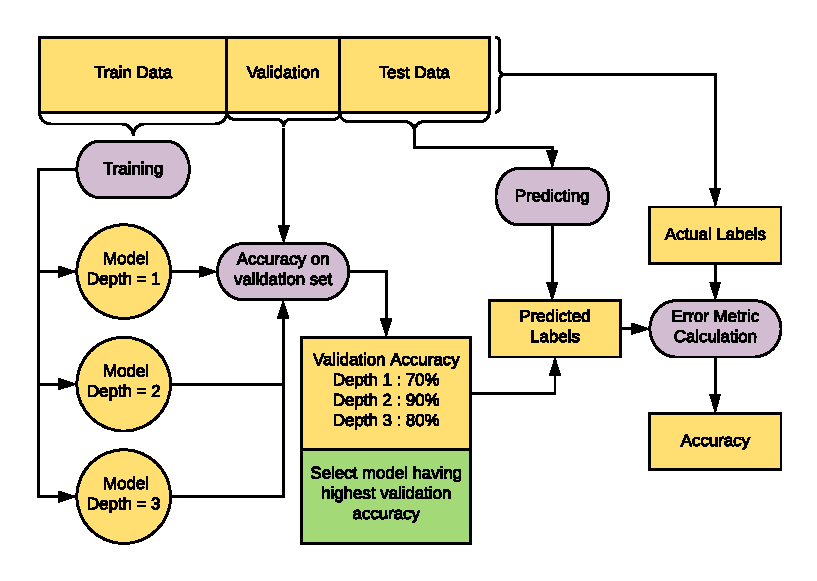
\includegraphics[width = \textwidth]{../diagrams/cross-validation/validation-workflow}
\end{frame}

\begin{frame}{Nested Cross Validation}
Divide your training set into $K$ equal 	parts.\\
Cyclically use 1 part as ``validation set" and the rest for training.\\
Here $K = 4$
\begin{center}
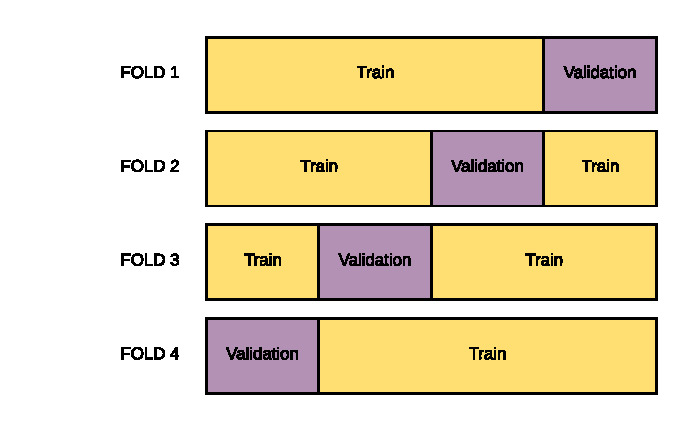
\includegraphics[scale=0.7]{../diagrams/cross-validation/cross-validation.pdf}
\end{center}
\end{frame}

\begin{frame}{Nested Cross Validation}
Average out the validation accuracy across all the folds\\
Use the model with highest validation accuracy\\
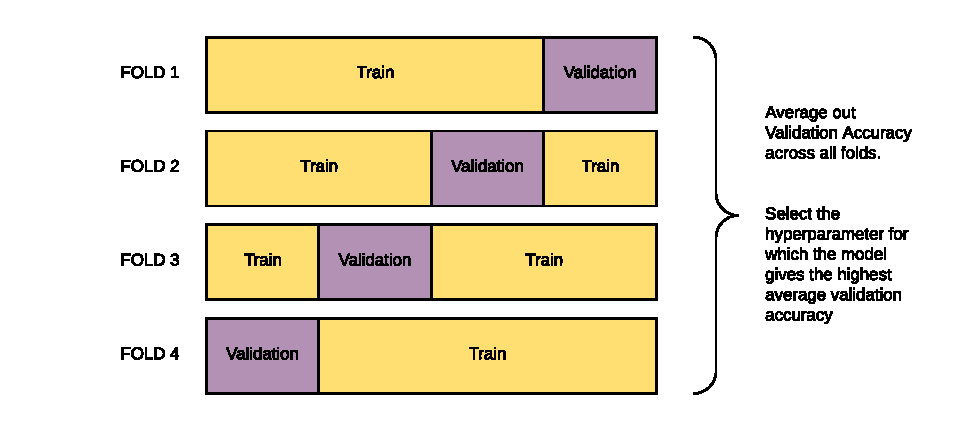
\includegraphics[width = \textwidth]{../diagrams/cross-validation/cross-validation-avg.pdf}
\end{frame}

\begin{frame}{Next time: Ensemble Learning}
\begin{itemize}
\item How to combine various models?
\item Why to combine multiple models?
\item How can we reduce bias?
\item How can we reduce variance?
\end{itemize}
\end{frame}

\end{document}